%file included in thesis.tex


\chapter{Data Representation and Interpretation}
\label{chap5}
The world representation should have a number of qualities. First it must represent the
world in a satisfactory way. It should be easy to update and take up little memory on the
implementation platform. Third it should be easy to understand for a human operator
without too much processing. 

It must be possible to determine the global position of the robot uniquely from the
observations the robot does during its mission. This can be achieved by matching the map
created only from observations to a map supplied by the user. This is a relatively easy
task when the both maps are of topological nature. The matching between those maps can
then be a graph search in the map supplied by the user. Depending on the accuracy of the
supplied map, the global position of the robot can be determined, and the path forward can
be chosen. 

In a topological world representation the geometrical aspect of a map is not that
important. Instead landmarks, interesting locations and other features which are easy 
recognizable are represented as nodes in a graph representation. 

Based on the terms that the world representation should not be spacious in memory, and
that exact distances are difficult to measure when there is no redundant global positioning
system, a topological world representation is pursued. 


\section{World Representation}
The world is classified into given nodes. Known features of the world is recognized
and represented as nodes in a graph. 

Possible environments must be stored in a database for the robot to be able to interpret
its surrounding. Said in another way, the robot must be taught its surroundings. 
This means that the world needs to be classified into predefined nodes before the mission
is started. A pipeline is a structured environment and can be divided into junctions. 

The nodes should have a number of attributes describing how the node is different from the
other nodes. These attributes are:
\begin{itemize}
    \item Node type
    \item Number
    \item Time stamp when discovered
    \item Previous Node
    \item Distance since last node
    \item Orientation
    \item Number of edges and the angles of those
    \item List of anomalies
\end{itemize}

\begin{figure}[htbp]
    \centering
    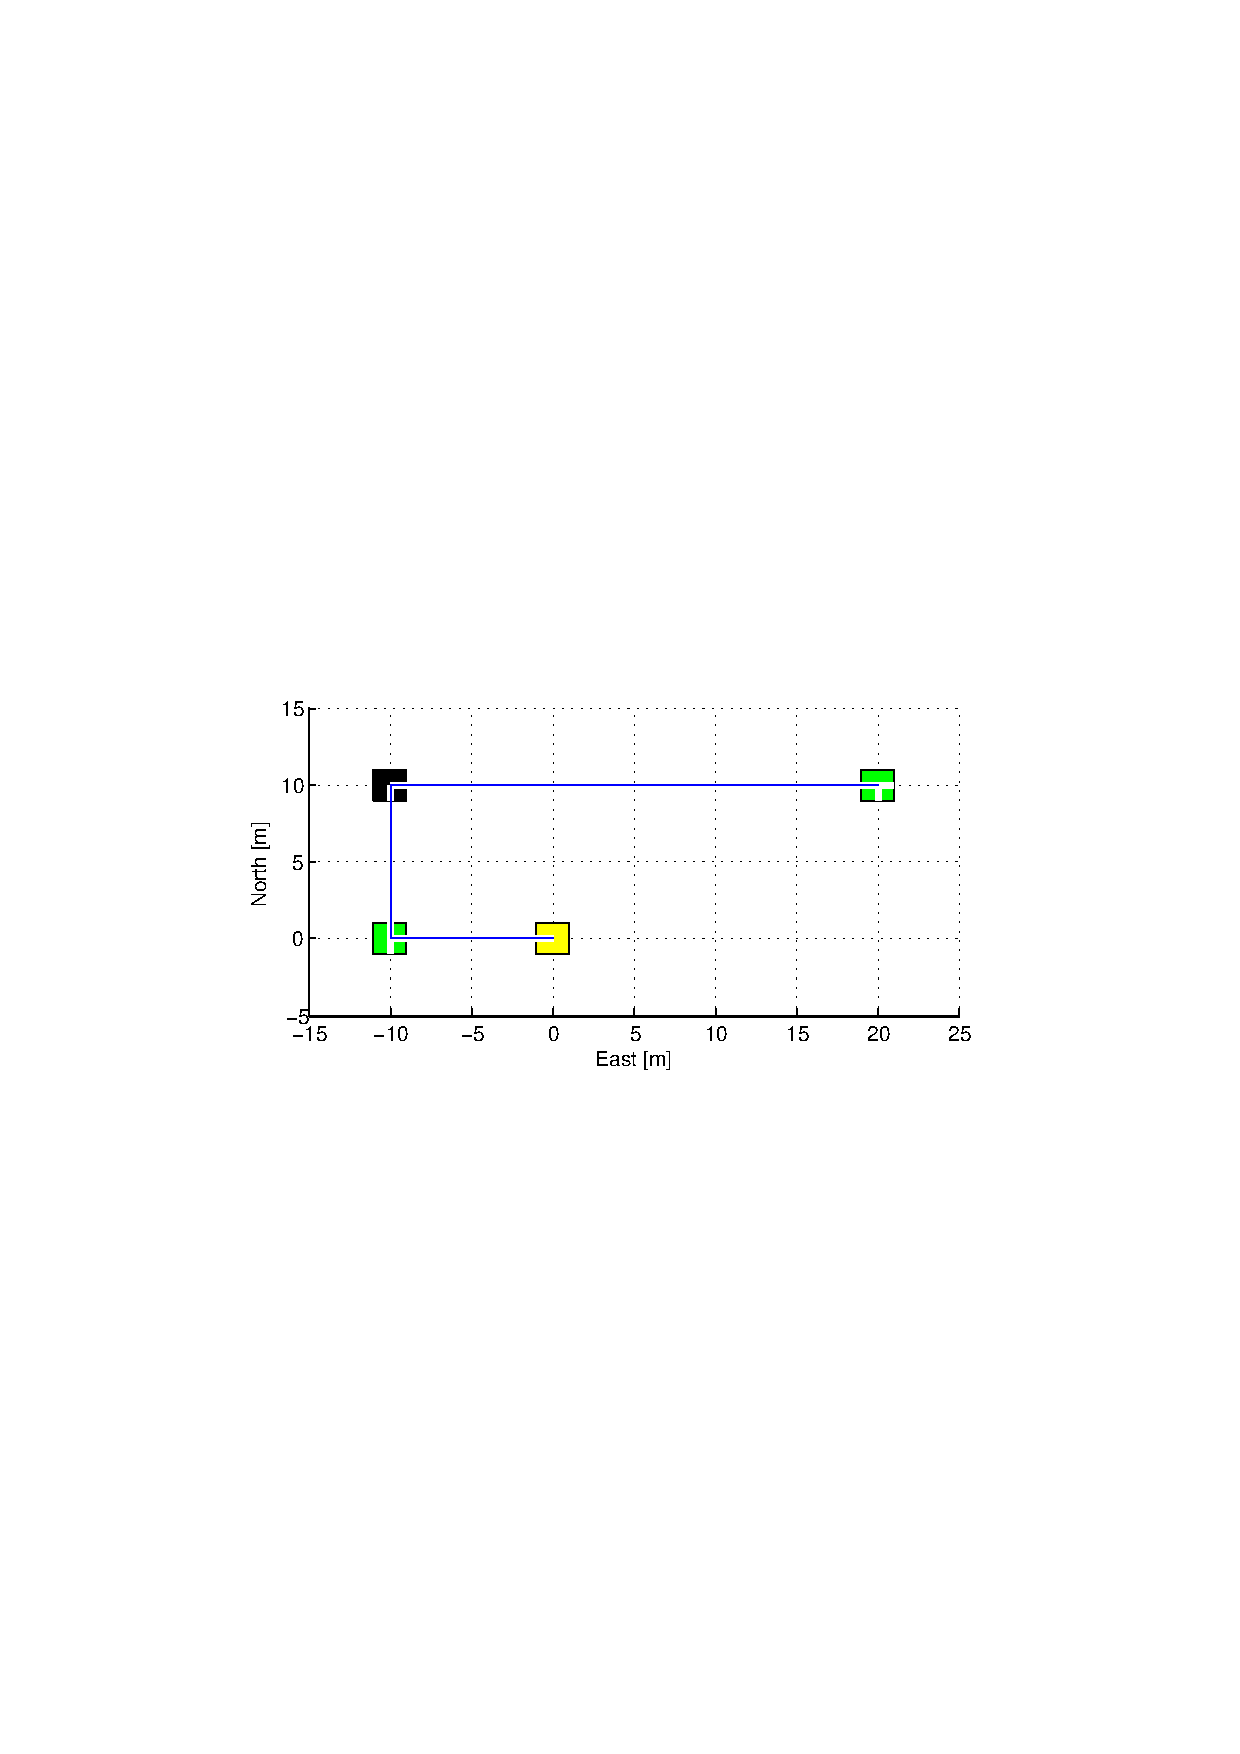
\includegraphics[width=0.8\textwidth]{pics/worldrepresentation}
    \caption{An example of the world representation}
    \label{chap5:fig-worldrepresentation}
\end{figure}
Most of this attributes are self-explaining, but the last attribute, \emph{list of
anomalies} deserves a closer explanation. 
Anomalies are those things that the robot should look after, and record. An anomaly is 
everything that is not expected. Everything that is not as expected should be recorded 
for later inspections. 

This list will contain every anomaly from the previous node to the next one, where the
list is stored. The list will contain a time stamp of when it was discovered, distance
travelled from the previous node, and a remark why it was detected as an anomaly. Since
this involves a lot of reasoning by the control system, there is a chance that actual
pipeline junctions might be marked as anomalies instead of being recognized as nodes.

Because the anomalies are detected before the node that will contain the list are
detected, the list is temporary stored in the robots memory until the next node are
detected. 

These anomalies might be obstacles which hinder the robot in completing its mission. It is
important that the control system is able to traverse these obstacles or take another way
to get past these obstacles. These special types of anomalies must be handled in some way
and should be marked as a node, but is not a topic of this project. 

\section{Map-building From the Sensor Data}
Much reasoning is needed from the control system to interpret the sensor data to select
and create the correct representation of the world, and more importantly take the correct
decisions when the robot is faced with a challenge. This part is maybe the most important
part in the complete navigation system, because it needs to supply correct information to
the higher level navigation and control system. If this part fails in assessing the
environment in the correct way, the navigation system might take the wrong decisions and
the entire mission might fail. 

To recognize nodes the sensors must be interpreted, and the output of this interpretation
needs to be matched to a database to determine what kind of node it is. 

\subsection{Interpreting 3D Sensor Data}
The point cloud output from the 3D sensors needs to be segmented to extract the features
which are of interest. 

The three dimensional point cloud which is output from the Time-of-Flight camera are
filtered before it is fed to the surface fit algorithm. Firstly the intensity images, is
used for filtering out pixels with too high or too low intensity values. The high
intensity values indicate that the pixel is too close to measure, or that the surface is
too reflective, either way this will give bad range data. The pixels which have too low
intensity values are either too far away, or might indicate that a multi-path reflections
and are filtered away. 

After doing this a number of successive captures are averaged to provide less noisy image.
Then the coordinates are sorted on the z-coordinate and divided into $n$ equally spaced
subsets. This means that there will be $n$ cylinders fitted to the captured point cloud.
This is too ease the amount of memory used to process the whole point cloud. 

The surface fit algorithm is a Nonlinear Least-Squares Guass-Newton algorithm. It
parameterizes the cylinder as described in Section \ref{chap2:sec-surface-fit-alg}. The input to this
algorithm is start coordinates of the cylinder axis, $x_0$, the direction cosines $a_0$, and
the initial radius, $r_0$.

\begin{algorithm}[htbp]
    \caption{Cylinder Fit Algorithm}
    \label{chap5:alg-cylinderfit}
    \begin{algorithmic}
        \REQUIRE (X, Y, Z) $\leftarrow$ point cloud and IntensityImage
        \STATE Filter pixels with intensity values below $LowIntensity$ and $HighIntensity$
        \STATE Average point cloud over $x$ samples
        \STATE Remove all trivial points
        \STATE Sort on Z-coordinate
        \STATE Divide point cloud into $n$ equally spaced $SubSets$
        \FOR{every $SubSets$}
            \STATE Get initial values for Surface Fit algorithm
            \STATE  $r, a, x_0, d$ $\leftarrow$ run surface fit algorithm on $SubSets$
        \ENDFOR
        \FOR{every $r_i$}
            \IF {$r_i > m \times PipeRadius$}
                \STATE Mark $r$ as erroneous
            \ENDIF
        \ENDFOR
    \end{algorithmic}
\end{algorithm}

There are a couple of problems. First, the points not belonging to the geographical
primitive, i.e. the cylinder will draw the cylinder fit off-axis, and cause the cylinder
fit to fail, as the Least-Squares approach assumes that all the points in the supplied set
belongs to the cylinder. 

The user parameters in this algorithm are the \emph{subset size} which decides the interval
of the subsets and also how many cylinders should be fitted to the given point cloud. The
other parameters are $m$ which tells for which values the predicted cylinder radii are
erroneous. 

The initial values which are required for the surface fit, is the assumed start position
of the cylinder which at the first \emph{SubSet} is at the origin with regard to the
ToF-camera sensor frame, and the initial axis which unless other is said is along the
z-axis, i.e. into the pipe seen from the camera.


\subsection{Interpreting 2D Sensor Data}
The laser range finder is the most accurate sensor on the platform. Therefore, this
sensor was selected to estimate the main direction and radius of the pipe. The sensor is
also limited to planar measurement, which limits the sensors ability to detect anomalies
in the pipeline; this is left to the 3D sensors. 

Line fit algorithm is a least-squares line fit algorithm. For this to work properly, a
selection of points assumed belonging to the line need to be fed into the algorithm. To
select these points a histogram is formed for both x- and y-direction of the points. This
will detect points which lie in a horizontal- and vertical lines. These points are selected
and fed into the line fit algorithm. 

It is assumed that the noise averages out when
enough samples are taken. Lines that are neither horizontal nor vertical
will cause problem for this algorithm. If the
histogram bins are too large, the direction of the fitted line will be diverted, and if it
is too small the algorithm will not detect the points as belonging to a line. 
\begin{algorithm}[htbp]
    \caption{2D Line Fit algorithm}
    \label{chap5:alg-2dlinefit}
    \begin{algorithmic}
        \REQUIRE $(r, \theta)$ from Laser Range Finder
        \STATE average $r, \theta$ over $n$ samples
        \STATE convert $r, \theta \rightarrow$ $x, y$ 
        \STATE with regard to $y$ construct histogram with $hist_y$ intervals
        \FOR{each $Bin$ in $HitogramY$}
            \IF{Number of points in $Bin$ $>$ $NoPointsY$}
                \STATE Pass these points to the Least-Squares Line Fit Alg $\rightarrow$ $a_y$, $b_y$
            \ENDIF
        \ENDFOR
        \STATE with regard to $x$ construct histogram with $hist_x$ intervals
        \FOR{each $Bin$ in $HitogramX$}
            \IF{Number of points in $Bin$ $>$ $NoPointsX$}
                \STATE Pass these points to the Least-Squares Line Fit Alg $\rightarrow$ $a_x$, $b_x$
            \ENDIF
        \ENDFOR
    \end{algorithmic}
\end{algorithm}

Parameters needed to be set by the user is, the histogram bin sizes, $hits_x$ and
$hits_y$. This controls the number of points that will be sorted into the bins. The bigger
the bins, the more vulnerable will the algorithm are to 
other points that do not ``belong'' to the wall points. Other parameters are the
threshold parameters for how many points there need to be in a histogram bin to pass them
to the line fit, $NoPointsX$ and $NoPointsY$.\

The horizontal lines, i.e. the ones that are along the $x$-axis shown in Figure
\ref{chap3:fig-sensor-frames}, are considered the most important, since these in most cases
are the walls of the pipeline. 

From these lines the radius and direction of the pipe can be found. The position of the
Laser Range finder is assumed known, particularly the height above the ground are needed
to calculate the radius of the pipe. The following relation is used.
\begin{align}
    r^2 &= P_2^2 + \left(\frac{d}{2} \right)^2 \\
    r &= P_1 + P_2  \quad \rightarrow \quad P_2 = r - P_1
\end{align}
Where $r$ is the radius of the pipe, $P_1$ is the distance from the measurement plane to
the lowest point in the pipe, $P_2$ is the distance from the center of the pipe to the
measurement plane and $d$ is the distance between the matched line segments. Substituting
for $P_2$ and rearranging
\begin{equation}
    \begin{aligned}
        r^2& = (r - P_1)^2 + \left(\frac{d}{2}\right)^2 = r^2 - 2 r P_1 + P_1^2 +
        \left(\frac{d}{2}\right)^2 \\
        2 r P_1 &= P_1^2 + \left(\frac{d}{2}\right)^2 \\
        r &= \frac{P_1}{2} + \frac{d^2}{8 P_1}
    \end{aligned}
\end{equation}
This requires that two lines can be matched to be approximately parallel for the distance
$d$ to be calculated. Therefore the direction of all the lines is compared to all the
other lines and those parallel within some threshold, $ParallelThreshold$ are selected.
These distances are compared to the \'a priori diameter of the pipe, inputted by the user. 

The estimated parameters here can be compared to the ones estimated from the 3D point
cloud, in a fashion that makes the system select the best estimate. The initial guess of
what sensor which provides the best results, are the laser range finder, which is
guaranteed to provide more accurate results from the manufacturer. The laser range finder
does also provide much less information to process, and will give results faster. 


\section{Matching Pipe Profiles and Detecting Anomalies}
Matching the pipe profiles is one of the central aspects when using this kind of abstract
representation. This method needs to be robust, and need to provide accurate results most
of the time.

First, the sensor data are processed and the pipeline properties are estimated, i.e.
radius and direction. This can be done using the laser range finder, which probably will
give the most accurate results, when around the robot. Then the \emph{misfit} points from
the 3D sensor is analysed, this can be matched to a database with \emph{fingerprints} of
the different pipeline junctions, and the best fit can be selected. \cite{sintef-tof}

The \emph{MRINSPECT-V} described in \cite{MRINSPECT-V} recognizes pipe profiles using the 
shadows created by a special illuminator. The shadow profiles are stored in tree
structure. Then a depth-first search can be used to find the matching profile fast and
efficient. 


Unfortunately, the profile matching has not been prioritized when working with this
project, and should be a topic of further research and work. 


\section{Navigation and Positioning in the World Representation}
How the control system determines the position in the environment is very important.
Because the system need to know where it is, and where it has been, to be
able to determine where it will go. 

Given the case that the system is capable of identifying and matching
the nodes correct, this can be used as landmark when determining global position. The
graph which has been created, can be matched with the \`a priori map, based on what kind
of nodes that have been passed. The path taken by the robot can be matched given that the
\`a priori map is accurate with regard to the location and order of the nodes. This is
similar to the approach used by the MAKRO project \cite{makro-visual}.

For example the robot passes first through an L-bend, then continues to a Y-Junction. It
continues to the left, where it hits an R-bend and into a T-Junction. This sequence of
nodes, can be matched to the given map, and a position can be estimated. If there are
ambiguities the correct position cannot be established before additional nodes are passed.
The pipe network needs to be, using an analogue to the system identification terminology, 
\emph{persistently exciting}. This means that the network consists of enough unique features and
sequences that the position can be determined uniquely. 

Further research and work is needed in this field to verify the proposed concept. 

